\chapter{Signed Distance Functions Techniques}\label{chp:LABEL_CHP_2}

A \textit{Signed Distance Function} (SDF) provides a way to describe geometric forms in a continuous manner by associating each point in space with its \textit{signed distance} to a surface. The function returns positive value when the point is outside the shape and a negative value when the point is inside the shape. This framework is highly flexible, allowing the representation of shapes in 2D, 3D, and even N-dimensional spaces, since the Euclidean distance is not restricted to a particular number of dimensions.  

A defining feature of Ray Marching is its use of signed distance functions to describe geometry, rather than traditional vertices, edges, and faces. This approach is precisely what makes Ray Marching a powerful technique, capable of rendering of smooth surfaces, shapes distorted by procedural noise, repetitive patterns, fractals, and dynamic shapes that evolve over time.
    
This chapter further describes signed distance functions for basic shapes and explores techniques for constructing complex shapes by combining and manipulating the fields to achieve the desired scene composition.

% https://www.shadertoy.com/view/lslXD8

\section{Basic Shapes}


The general form of an SDF function includes:  

\begin{itemize}
    \item $\mathbf{p}$, the \textbf{query point}, for which the distance from the shape positioned at the origin is computed.
    \item Shape-specific parameters, such as the \textbf{radius} for circles and spheres, or additional properties like \textbf{width, height, or orientation} for more complex geometries.
\end{itemize}

\subsection{Circles and Spheres}

For a circle centered at the origin in $ \mathbb{R}^ 2 $ with radius $r$, the SDF is given by:

$$\text{CircleSDF}(\mathbf{p}) = \|\mathbf{p}\| - r$$

A sphere in three-dimensional space follows the same principle. If the sphere is centered at the origin with radius $r$, the SDF becomes:

$$\text{SphereSDF}(\mathbf{p}) = \|\mathbf{p}\| - r$$


where $\mathbf{p}$ in $\mathbb{R}^3 $ is now a point in three-dimensional space.

The only difference between the circle and the sphere is the dimension of the query point $\mathbf{p}$. In the case of a circle, $\mathbf{p}$ is a two-dimensional vector, whereas for a sphere, $\mathbf{p}$ is a three-dimensional vector. The formula remains structurally identical because both objects are defined by a center and a radius in their respective spaces.

\begin{lstlisting}[language=GLSL, caption={Code 2: Circle and Sphere SDFs}, label={lst:CircleAndSphere} float=H]
float circleDistance(vec2 point, float radius){
    return length(point) - radius;
}

float sphereDistance(vec3 point, float radius){
    return length(point) - radius;
}
\end{lstlisting}

Since an SDF returns a positive distance when a point is outside the primitive and a negative distance when inside, this information can be used to assign different colors to a 2D shape rendered on the canvas.

\begin{lstlisting}[language=GLSL, caption={Code 3: Rendering Circles}, label={lst:ColoringCircle} float=H]
vec3 plainColor (in float d){
     return vec3(1.0) - sign(d)*vec3(0.4);
}

void mainImage( out vec4 fragColor, in vec2 fragCoord )
{
    vec2 uv = (2.*fragCoord.xy-iResolution.xy)/min(iResolution.x, iResolution.y);

    float d = circleDistance(uv, 0.5);

    vec3 col = plainColor(d);
    fragColor = vec4(col,1.0);
}
\end{lstlisting}

\begin{figure}
\centering
\begin{minipage}{.5\textwidth}
  \centering
  
\includegraphics[width=.8\linewidth]{imagens/circle-plainColor.png}
  \captionof{figure}{Plain Colored Circle}
  \label{fig:plainColoredCircle}
\end{minipage}%
\begin{minipage}{.5\textwidth}
  \centering
  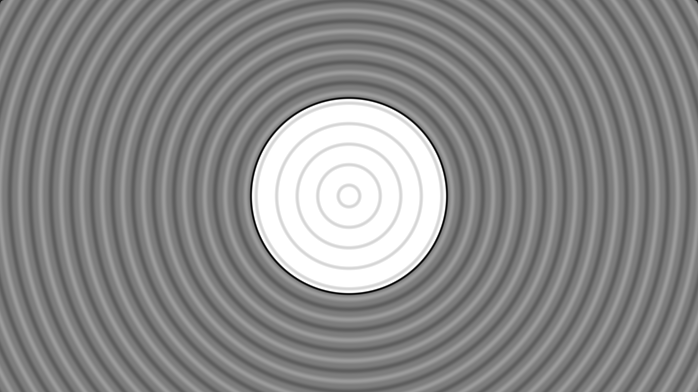
\includegraphics[width=.8\linewidth]{imagens/circle-customColor.png}
  \captionof{figure}{Custom Colored Circle}
  \label{fig:customColoredCircle}
\end{minipage}
\end{figure}

In Figure \ref{fig:plainColoredCircle}, it is possible to see the color outside the circle being rendered in a darker shade than inside the circle. The implementation for such render can be seen in Code 3. For the following shapes, we will use a custom coloring function that adds isolines and highlights the border, as shown in Figure \ref{fig:customColoredCircle}. This technique allows the visualization of 2D SDFs in the distance space.

3D Signed Distance Functions (SDFs) define the shapes of objects within a scene in the Ray Marching pipeline. For instance, the distance function of a sphere can represent the scene's minimum distance in the \texttt{createScene} function (see Code 1). Rays are marched accordingly, and collision information is passed to the \texttt{getHitColor} function. As previously discussed, this process closely resembles both Ray Marching and Ray Tracing techniques, including the lighting calculations used to shade the hit point. The following examples in this chapter illustrate 3D SDFs rendered with Lambertian diffuse shading and Phong specular reflection.

\begin{figure}[ht]
    \centering
  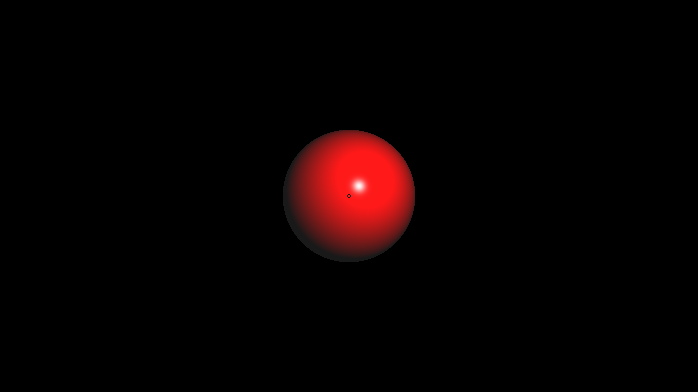
\includegraphics[width=.6\linewidth]{imagens/sdf-sphere.png}
  \captionof{figure}{Raymarched Sphere SDF Visualization}
  \label{fig:sdf-sphere}
\end{figure}

Since lighting models are outside the scope of this essay, readers may refer to Real-Time Rendering, 4th Edition by Akenine-Möller et al. for further details on shading techniques \cite{akenine-moller2018realtimerendering}.

\subsection{Rectangles and Boxes}

% \begin{figure}[ht]
%     \centering
%   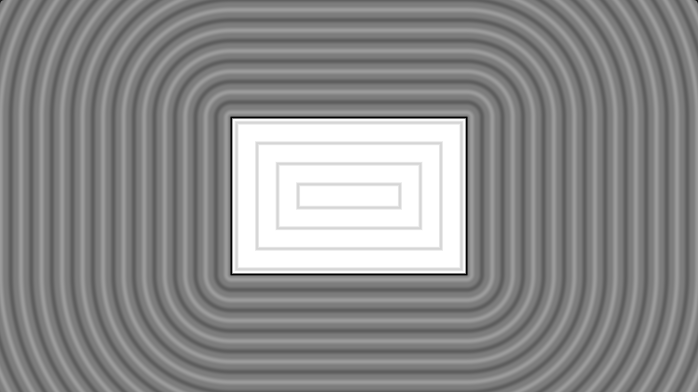
\includegraphics[width=.6\linewidth]{imagens/rectangle-customColor.png}
%   \captionof{figure}{Rectangle SDF Visualization}
%   \label{fig:customColoredRectangle}
% \end{figure}

Similar to the 2D circle, the signed distance function (SDF) of a 2D box, or rectangle, can be generalized to higher dimensions.

\begin{lstlisting}[language=GLSL, caption={Code 4: Rectangle and Box SDF}, label={lst:RectangleAndBox} float=H]
float rectangleDistance( in vec2 p, in vec2 b ){
    vec2 d = abs(p)-b;
    return length(max(d,0.0)) + min(max(d.x,d.y),0.0);
}

float boxDistance( in vec3 p, in vec3 b ){
    vec3 d = abs(p)-b;
    return length(max(d,0.0)) + min(max(d.x,d.y,d.z),0.0);
}
\end{lstlisting}

The rectangle SDF is defined at the origin $\mathbf{[0,0]}$, and due to the rectangle's symmetry, it is often more convenient to work within the first cartesian quadrant. To achieve this, $\mathbf{b}$ (half each box`s side) is subtracted from $\mathbf{abs(p)}$, yielding a point $\mathbf{d}$. As illustrated in Figure \ref{fig:square_sdf}:

\begin{itemize}
    \item If only $\mathbf{d.x<0}$, it indicates that $\mathbf{p}$ is above the rectangle, in section 1, and the shortest distance is straight down.
    \item If only $\mathbf{d.y<0}$, it means that $\mathbf{p}$ is next to the rectangle, in section 3, so the shortest distance is straight left.
    \item If both $\mathbf{d.x}<0$ and $\mathbf{d.y<0}$, the point is inside the rectangle, in section 4, thus the shortest distance is the closest of the two sides.
    \item Finally, if neither component is negative, the point lies diagonally outside the rectangle, in section 2, so the distance to the corner is the shortest.
\end{itemize}

\begin{figure}[ht]
    \centering
    \fbox{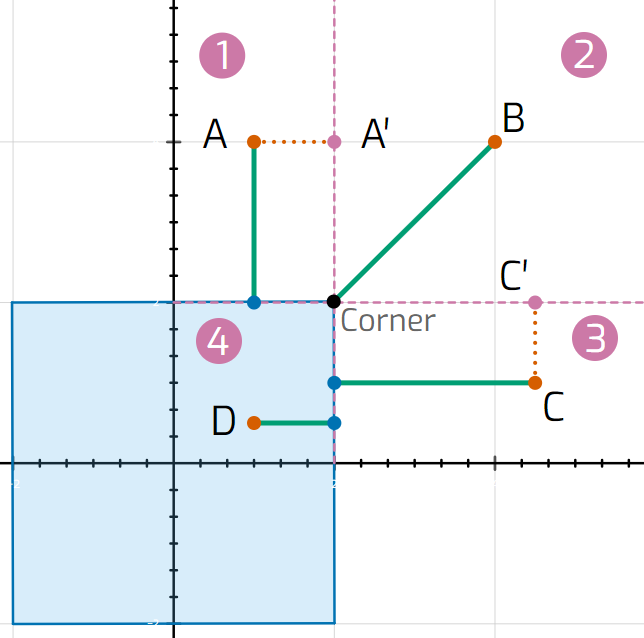
\includegraphics[width=7.5cm,height=7.43cm]{imagens/square_sdf.png}}
    \caption{Graphic of Rectangle SDF calculation}
    \label{fig:square_sdf}
\end{figure}

It can be seen that when both $\mathbf{d.x}$ and $\mathbf{d.y}$ are limited to zero, which visually means snapping all points to section 2, the distance to the corner encases the results, although not entirely. If in section 4, inside the rectangle, $\mathbf{length(max(d,0.0))}$ is always 0. In such cases, the SDF should return the negative distance to the nearest edge of the rectangle, adding the expression $\mathbf{min(max(d.x,d.y),0.0)}$. The min() function ensures non-zero distances are only possible in section 4. With that, all sections are considered.

This process can be generalized to higher dimensions in a similar fashion. As such, the 3D box SDF can be derived by extending the approach to $\mathbb{R}^3 $, where p and b are now three-dimensional vectors.


\begin{figure}[ht]
    \centering
  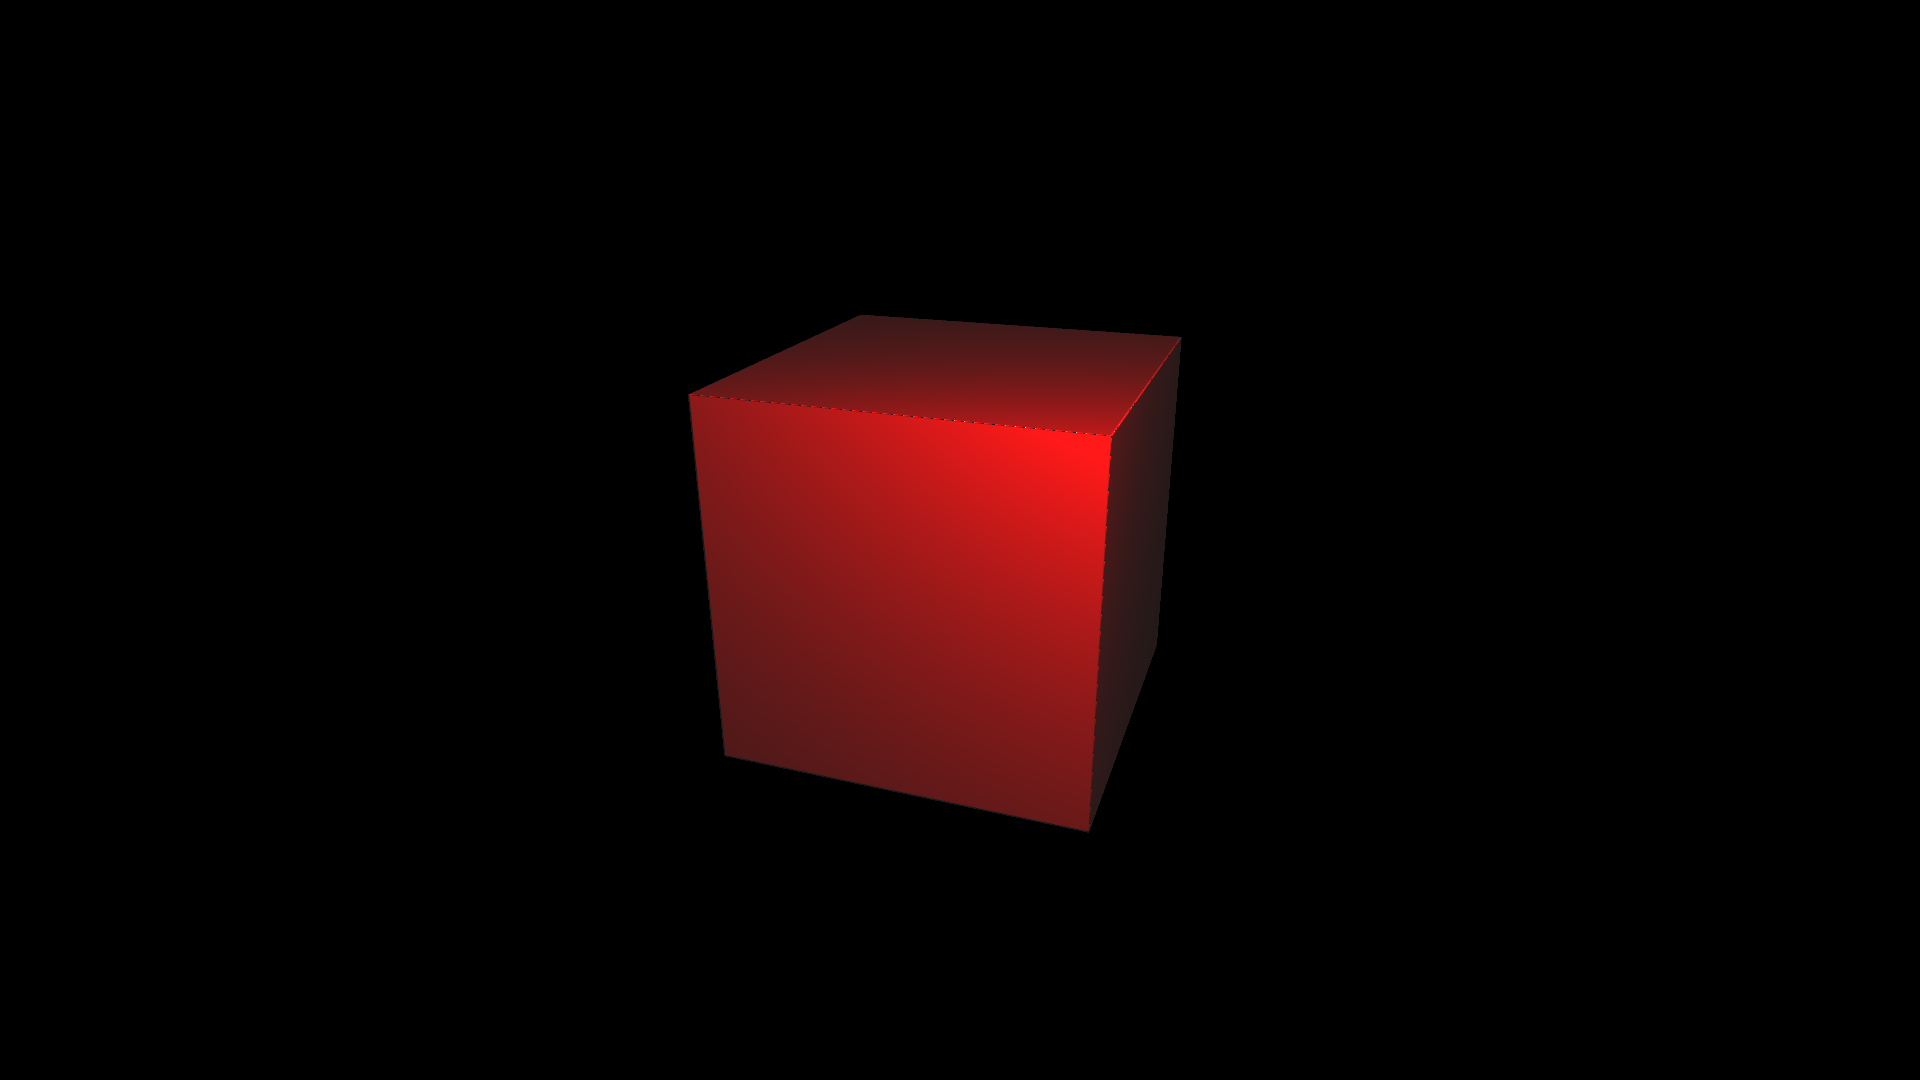
\includegraphics[width=.6\linewidth]{imagens/sdf-cube.png}
  \captionof{figure}{3D Cube SDF Visualization}
  \label{fig:sdf-cube}
\end{figure}


If expanded to $\mathbb{R}^4 $, the SDF can help visualize forms such as the tesseract, the 4D hypercube, by fixing and scrolling through one of the four axes.

\section{Basic Transformations}

All primitive described in the previous section were centered at the origin. In order to perform a transformation such as scaling, rotation or translation, it is possible to apply the transformation at the query point $\mathbf{p}$.

%BOTAR EXEMPLO DE CODIGO FACIL
%vec3 opTransformRotate( in vec3 p, in transform t, in sdf3d primitive ){
%    return primitive( invert(t)*p );
%}
%float opScale( in vec3 p, in float s, in sdf3d primitive ){
%    return primitive(p/s)*s;
%}

%UM PARAGRAFO PRA EXPLICAR RAPIDINHO

\section{Operations}

While being able to display a variety of primitives is great, both ray tracing and ray marching have such capabilities. As time goes by, what is required of modern computer graphics becomes much more than that, and in search of building more complex forms is where both methods part ways. While ray tracing depends on high polygon-count models, almost never using other types of primitives, ray marching finds more success with a variety of solutions, one such being the use of various combinations between primitives and operations as building blocks.
This section describes some of the main SDF operations used in modeling based on basic primitives. Having primitives centered at the origin also facilitates many of the operations.

\subsection{Union, Intersection and Subtraction}

Operations between objects are some of the most elegant features of SDFs, and the most basic ones are the combinations: Union, Intersection and Subtraction. These three have very simple definitions and are great ways to introduce SDF operations. They take as input the SDF resulting distance of two primitive SDFs.


\begin{lstlisting}[language=GLSL, caption={Code 5: SDF Union, Intersection and Subtraction}, label={lst:UnionIntersectionSubtraction} float=H]
float unionOperation( float d1, float d2 )
{
    return min(d1,d2);
}
float intersectionOperation( float d1, float d2 )
{
    return max(d1,d2);
}
float subtractionOperation( float d1, float d2 )
{
    return max(-d1,d2);
}
\end{lstlisting}

From the perspective of a 3D raymarched vision, given $\mathbf{d1}$ and $\mathbf{d2}$, SDF distances from objects 1 and 2:

\begin{itemize}
    \item Taking the minimum between $\mathbf{d1}$ and $\mathbf{d2}$ is like seeing only the closest surface from both objects to camera, which is already the case for solids seen from the outside.
    \item Taking the maximum between $\mathbf{d1}$ and $\mathbf{d2}$ means that nothing outside the intersection of both objects is seen, since the ray march will only consider a hit if both SDF results are below the hit threshold.
    \item Taking the maximum between $\mathbf{-d1}$ and $\mathbf{d2}$ is like intersecting with the inverse of d1, which means that all $\mathbf{R}^3 $ except object1. This results in the subtraction of objects 1 from 2.
\end{itemize}


\begin{figure}[h!]
    \centering

    % Row 1
    \begin{minipage}{0.3\textwidth}
        \centering
        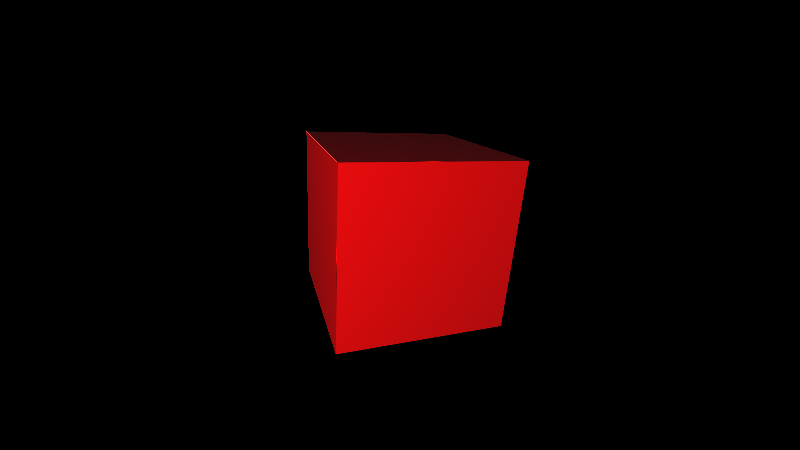
\includegraphics[width=\linewidth]{imagens/sdf-operations/cube.png}\\
        Cube
    \end{minipage}%
    \hfill
    \begin{minipage}{0.3\textwidth}
        \centering
        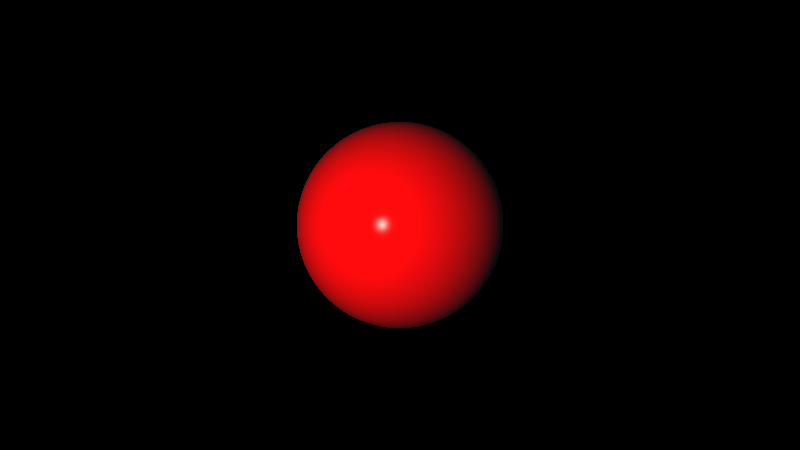
\includegraphics[width=\linewidth]{imagens/sdf-operations/sphere.png}\\
        Sphere
    \end{minipage}%
    \hfill
    \begin{minipage}{0.3\textwidth}
        \centering
        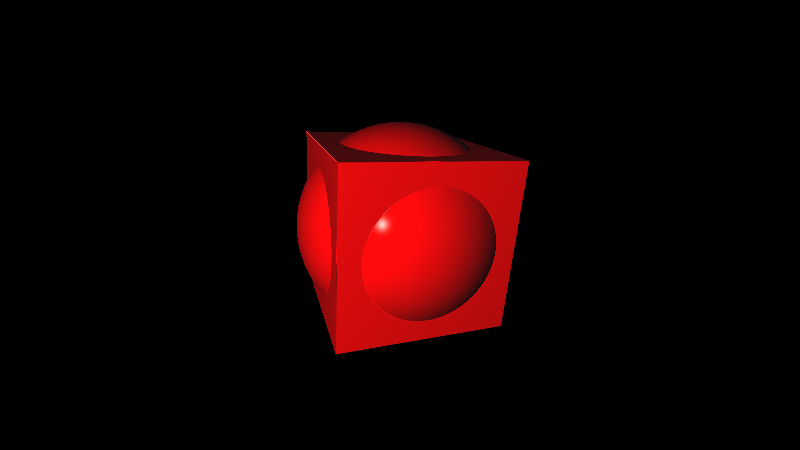
\includegraphics[width=\linewidth]{imagens/sdf-operations/union.png}\\
        Union
    \end{minipage}

    \vspace{1em} % space between rows

    % Row 2
    \begin{minipage}{0.3\textwidth}
        \centering
        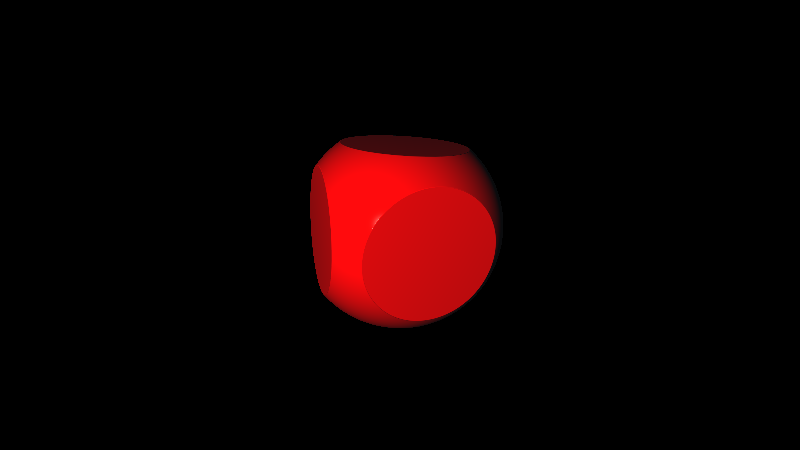
\includegraphics[width=\linewidth]{imagens/sdf-operations/intersection.png}\\
        Intersection
    \end{minipage}%
    \hfill
    \begin{minipage}{0.3\textwidth}
        \centering
        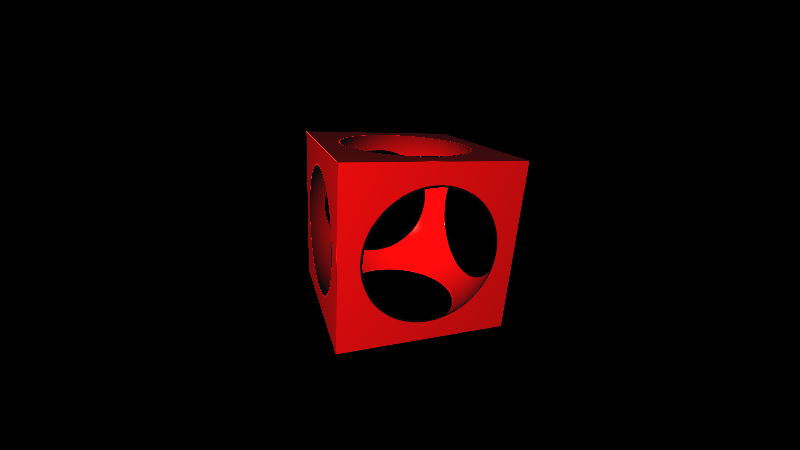
\includegraphics[width=\linewidth]{imagens/sdf-operations/subtraction1.png}\\
        Subtraction 1
    \end{minipage}%
    \hfill
    \begin{minipage}{0.3\textwidth}
        \centering
        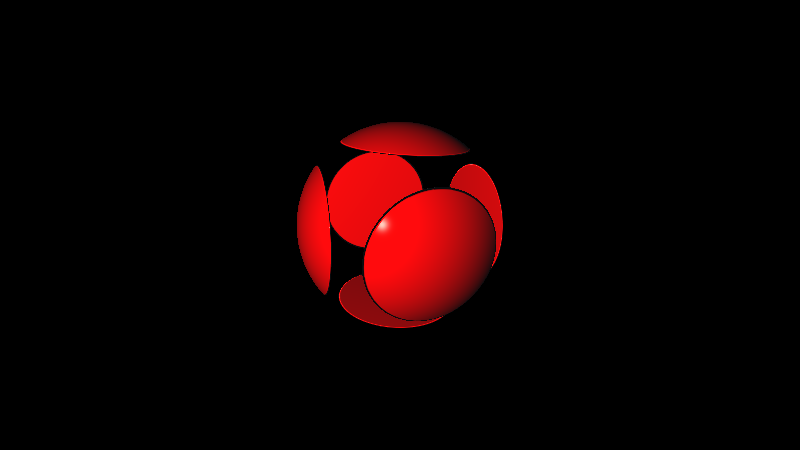
\includegraphics[width=\linewidth]{imagens/sdf-operations/subtraction2.png}\\
        Subtraction 2
    \end{minipage}

    \caption{Raymarched Constructive Solid Geometry Operations with Cube and Sphere SDFs.}
    \label{fig:sdf_operations}
\end{figure}

\subsection{Smooth Union, Intersection and Subtraction}

A more complicated, yet visually appealing way to display the basic boolean operations is through the use of Smooth Minimum and Maximum. As the name implies, instead of binary hard edge transitions between the primitives, it offers a smooth blend. Figures \ref{fig:sunion}, \ref{fig:sinter} and \ref{fig:ssub} combine the same box and circle with each smooth variant of the basic operations.
This blending can be achieved through multiple types of functions, such as quadratic, cubic, exponential, sigmoid, each having it`s pros and cons.

\begin{figure}
\centering
\begin{minipage}{.5\textwidth}
  \centering
  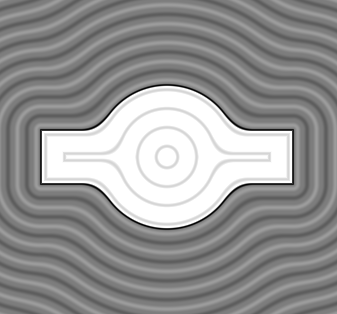
\includegraphics[width=.8\linewidth]{imagens/smoothUnion.png}
  \captionof{figure}{Smooth Union}
  \label{fig:sunion}
\end{minipage}%
\begin{minipage}{.5\textwidth}
  \centering
  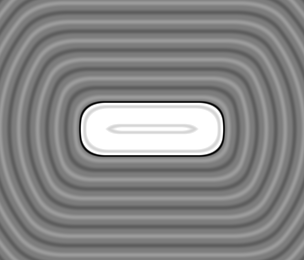
\includegraphics[width=.8\linewidth]{imagens/smoothIntersection.png}
  \captionof{figure}{Smooth Intersection}
  \label{fig:sinter}
\end{minipage}
\end{figure}
\begin{figure}
\centering
\begin{minipage}{.5\textwidth}
  \centering
  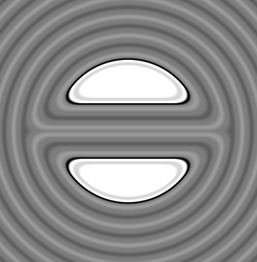
\includegraphics[width=.8\linewidth]{imagens/smoothSubtraction.png}
  \captionof{figure}{Smooth Subtraction}
  \label{fig:ssub}
\end{minipage}%
\begin{minipage}{.5\textwidth}
  \centering
  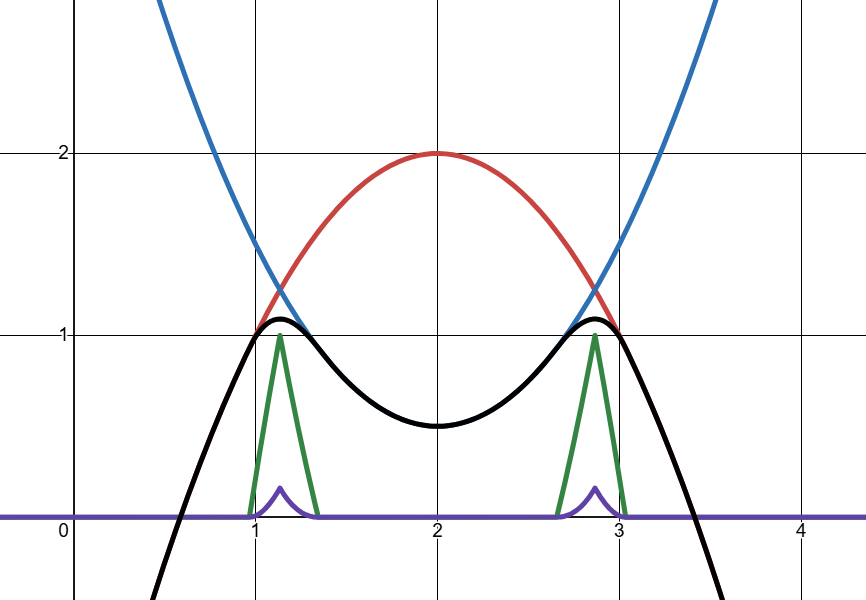
\includegraphics[width=.8\linewidth]{imagens/desmos_smin.png}
  \captionof{figure}{Smooth Minimum Representation}
  \label{fig:smin}
\end{minipage}
\end{figure}

Because it is fast and does not overestimate distances, the quadratic polynomial is less prone to visual artifacts and is the most widely used version for ray marching, thus being the one this section focuses on. Similarly to the regular min function, smin (smooth minimum) takes as input $\mathbf{a}$ and $\mathbf{b}$, which could be distances, or points in space, plus the threshold $\mathbf{k}$. The blending starts where the distance between $\mathbf{a}$ and $\mathbf{b}$ is smaller than $\mathbf{k}$.

Figure \ref{fig:smin} will help navigate the explanation ahead, $\mathbf{a\ =\ -\left(2-x\right)^{2}+2}$ is in red and $\mathbf{b\ =\ \left(2-x\right)^{2}\ +.5}$ in blue. To find smin, all polynomial methods start by finding the $\mathbf{h()}$ function, which is 0 by default, and ramps up to 1, starting at $\mathbf{|a - b|=k}$ and peaking at $\mathbf{|a - b|=0}$:

\begin{equation}
    h = \frac{\max(k - |a - b|, 0.0)}{k}
    \label{eq:example_equation}
\end{equation}

Since $\mathbf{k}$ is the distance in which the shapes start to combine, $\mathbf{h()}$ helps delimitate exactly that, as represented in green, Figure \ref{fig:smin}. Next, there needs to be a $\mathbf{c}$ such that $\mathbf{min(a,b)-c}$ produces the smoothed curve. This is no random requirement, but a simplified structure of what is the DD (Direct Difference) family of smin solutions. For polynomials, a simple solution for $\mathbf{c}$ is as follows, with $\mathbf{n>1.5}$ already producing great results:

\begin{equation}
    c\ =\frac{h^{n}k}{2n}
    \label{eq:example_equation}
\end{equation}

Between all values of $\mathbf{n}$, the quadratic version ($\mathbf{n=2}$) produces the gentler of curves, and is prioritized over the others. To better visualize what $\mathbf{c}$ means, Figure \ref{fig:sunion} represents $\mathbf{c}$ in purple. Squaring $\mathbf{h}$ makes c ease into 1, instead of following a straight ramp. Multiplying by $\mathbf{k}$ compensates any variation, as the peak of $\mathbf{h}$ decreases as $\mathbf{k}$ increases. Lastly, the divisor helps position the peak to the right place.
To achieve smooth maximum, all that is needed is $\mathbf{max(a,b)+c}$.

\begin{figure}[h!]
    \centering

    % Row 1
    \begin{minipage}{0.3\textwidth}
        \centering
        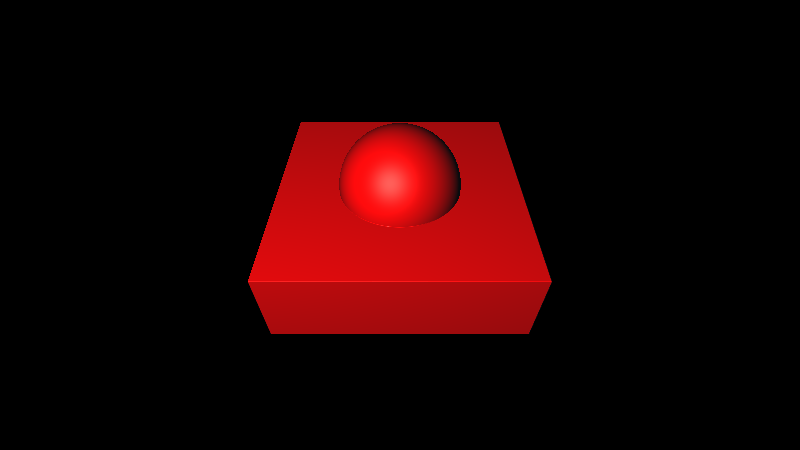
\includegraphics[width=\linewidth]{imagens/smooth-sdf-operations/add-unsmooth.png}\\
        Addition
    \end{minipage}%
    \hfill
    \begin{minipage}{0.3\textwidth}
        \centering
        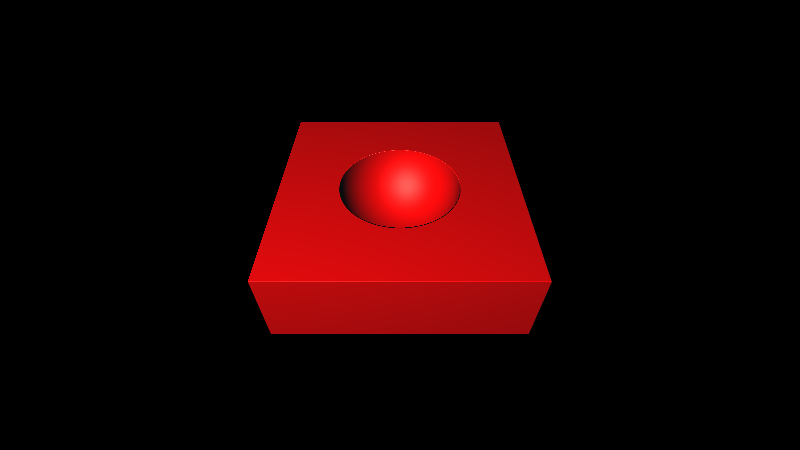
\includegraphics[width=\linewidth]{imagens/smooth-sdf-operations/subtraction-unsmooth.png}\\
        Subtraction
    \end{minipage}%
    \hfill
    \begin{minipage}{0.3\textwidth}
        \centering
        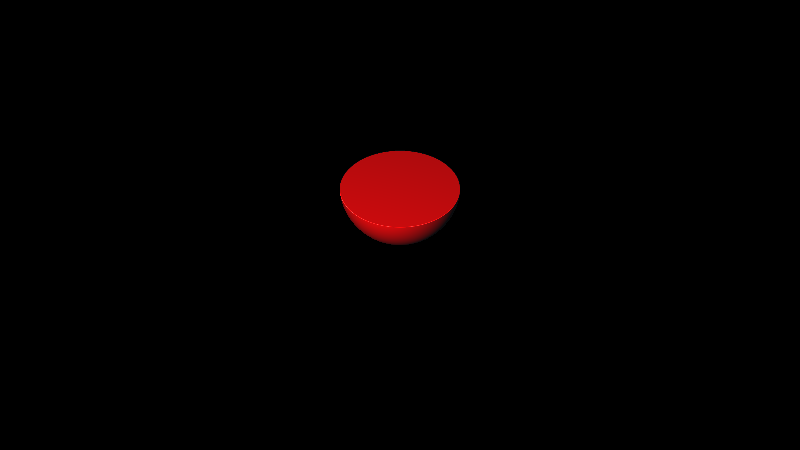
\includegraphics[width=\linewidth]{imagens/smooth-sdf-operations/intersection-unsmooth.png}\\
        Intersection
    \end{minipage}

    \vspace{1em} % space between rows

    % Row 2
    \begin{minipage}{0.3\textwidth}
        \centering
        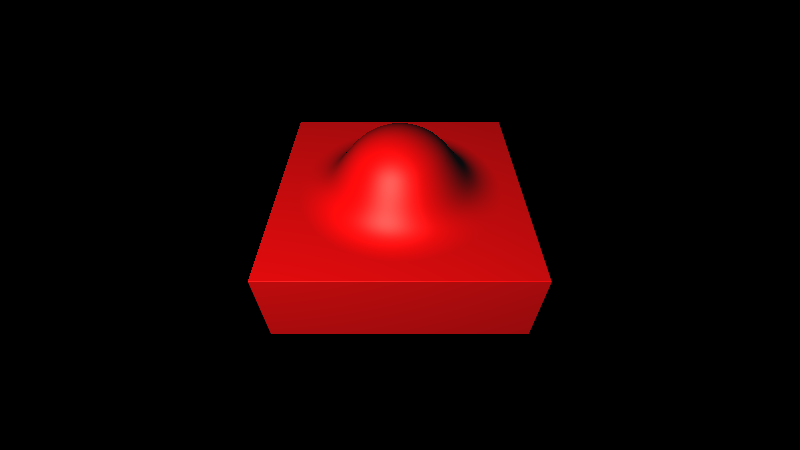
\includegraphics[width=\linewidth]{imagens/smooth-sdf-operations/add-smooth.png}\\
        Smooth Addition
    \end{minipage}%
    \hfill
    \begin{minipage}{0.3\textwidth}
        \centering
        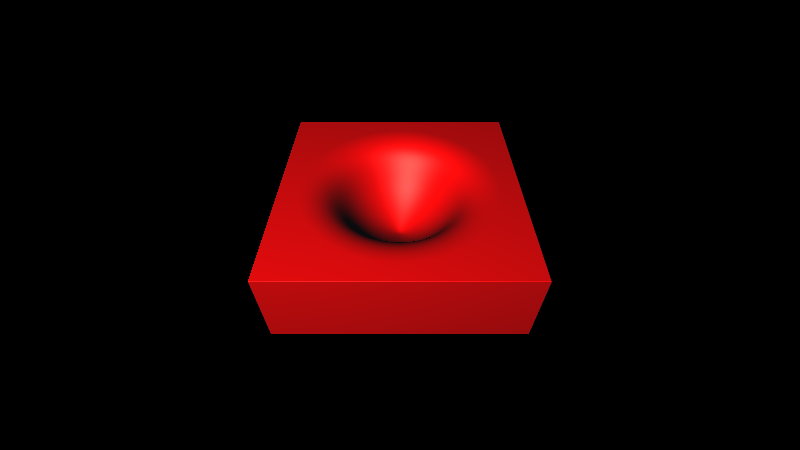
\includegraphics[width=\linewidth]{imagens/smooth-sdf-operations/subtraction-smooth.png}\\
        Smooth Subtraction
    \end{minipage}%
    \hfill
    \begin{minipage}{0.3\textwidth}
        \centering
        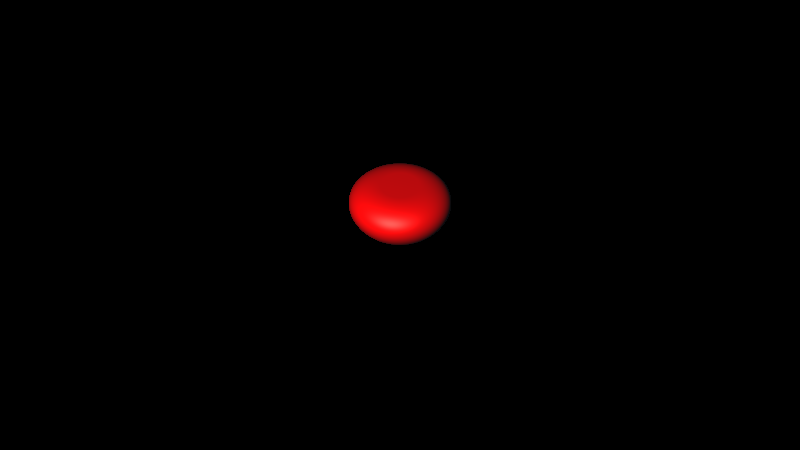
\includegraphics[width=\linewidth]{imagens/smooth-sdf-operations/intersection-smooth.png}\\
        Smooth Intersection
    \end{minipage}

    \caption{Raymarched Smooth Operations with Cube and Sphere SDFs.}
    \label{fig:smooth_sdf_operations}
\end{figure}

\subsection{Domain Repetition}

Since SDFs are expressed as mathematical functions, they can be transformed to repeat periodically across space. This technique, known as domain repetition, allows for the creation of infinite, repeating patterns in a scene while also optimizing performance by avoiding the need for multiple individual primitives.

There are many variations of this technique, as any domain parametrization can be made repeating, but the core idea is to use mathematical operations that will result in the desired scene. 

This can be achieved through the natural repetitive pattern of trigonometric functions such as $sin(x)$ and $cos(x)$, however, bending the domain with these functions will compromise the accurate Euclidean distances of the space the SDFs relies on, and this might generate unwished features. Functions such as $round(x)$ or $mod(x)$ (modulus operator) are more commonly used instead.

\begin{figure}[h!]
    \centering

    % Row 1
    \begin{minipage}{0.45\textwidth}
        \centering
        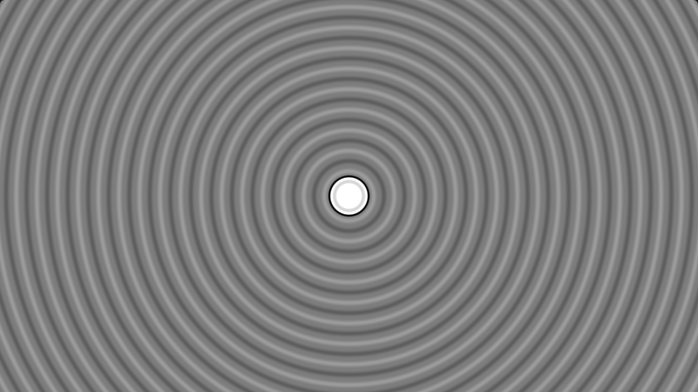
\includegraphics[width=\linewidth]{imagens/domainRepetition-circle.png}\\
        circleDistance(uv, 0.1)
    \end{minipage}%
    \hfill
    \begin{minipage}{0.45\textwidth}
        \centering
        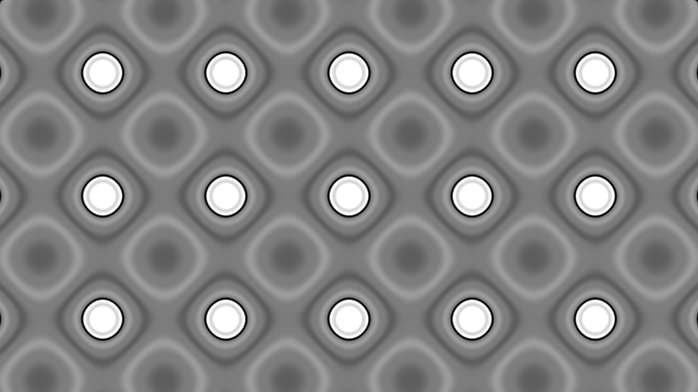
\includegraphics[width=\linewidth]{imagens/domainRepetition-sine.png}\\
        circleDistance(sin(uv * 5.)*0.2, 0.1)
    \end{minipage}

    \vspace{1em} % space between rows

    % Row 2
    \begin{minipage}{0.45\textwidth}
        \centering
        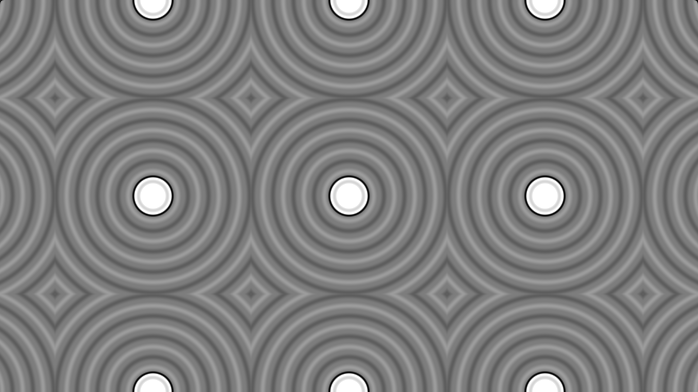
\includegraphics[width=\linewidth]{imagens/domainRepetition-round.png}\\
        circleDistance(uv - round(uv), 0.1)
    \end{minipage}%
    \hfill
    \begin{minipage}{0.45\textwidth}
        \centering
        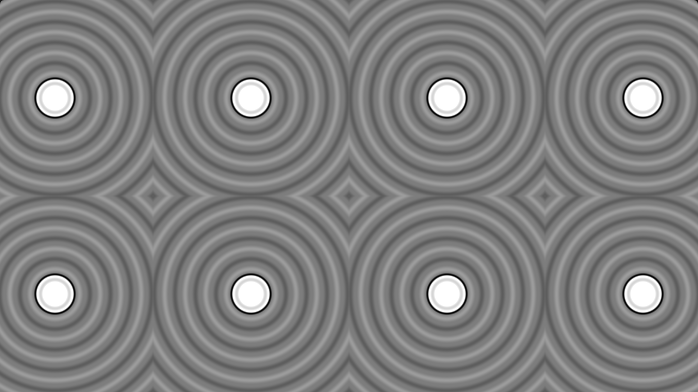
\includegraphics[width=\linewidth]{imagens/domainRepetition-mod.png}\\
        circleDistance(mod(uv, 1.)-0.5, 0.1)
    \end{minipage}

    \caption{Examples of Domain Repetition techniques.}
    \label{fig:domainRepetition}
\end{figure}

Given that \textbf{uv} represents the query point in the domain, with the zero vector centered on the canvas, Figure \ref{fig:domainRepetition} illustrates the output of the custom coloring function applied to its respective transformation. Naturally, this can also be used in 3D: Given that $\mathbf{p}$ represents the query point in the domain, the repeated domain can be represented as 
$\mathbf{p} - \textit{gap} \cdot \mathrm{round}\!\left( \frac{\mathbf{p}}{\textit{gap}} \right)$,
where \textit{gap} is the size of the repeated domain box. Figure~\ref{fig:sdf-3d-domainRepetition} 
shows an example of repeated spheres in a repeated domain.

\begin{figure}[ht]
    \centering
  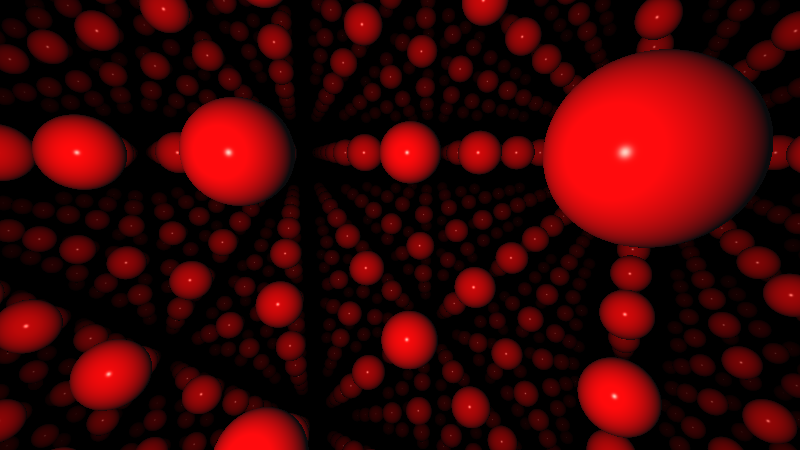
\includegraphics[width=.6\linewidth]{imagens/domain-repetition.png}
  \captionof{figure}{sphereDistance(p - 6.5*round(p/6.5), 1.0)}
  \label{fig:sdf-3d-domainRepetition}
\end{figure}

\subsection{Displacement}

Displacement is a technique used to adjust the geometry to simulate bumps or irregularities, adding fine detail to the surface. This is often done by perturbing the distance field using patterns that look random, such as static or grain, which can be generated with mathematical formulas (procedural noise) or taken from images (noise textures).

\begin{lstlisting}[language=GLSL, caption={Code 6: SDF Displacement}, label={lst:Displacement} float=H]
float displacementOperation( in sdf3d sdfShape, in vec3 p )
{
    float d1 = sdfShape(p);
    float d2 = displacement(p);
    return d1+d2;
}
\end{lstlisting}

Although noisy functions are commonly used for displacement, any function can be applied to distort the distance field. This flexibility enables the creation of non-Euclidean effects, such as bending or twisting space. However, this comes with a caveat: the sum of an SDF and an arbitrary function is not necessarily an SDF.

A key property of 2D and 3D Signed Distance Functions is that their gradient has length $1.0$ everywhere in the space. Since SDFs measure distances, the rate of change of distance must be equal to 1.0. When two SDFs are added, this property is violated — the gradient no longer has unit length, effectively "bending" space. This can cause the raymarcher to underestimate or overestimate the true distance from the surface.

This issue can be attenuated by reducing the step size and increasing the number of marching iterations, though this comes at a performance cost. In practice, small deviations in the length of the gradient rarely produce noticeable artifacts, making displacement through function addition still useful for subtle surface displacement.

\begin{lstlisting}[language=GLSL, caption={Code 7: Wave Distortion on Sphere}, label={lst:DistortionOnSphere} float=H]
float distortedSphereDistance(vec3 p){
    float sphereRadius = 2.0;
    vec3 sphereCenter = vec3(0., 2., -5.);
    float sphereDist = length(p - sphereCenter) - sphereRadius;

    vec2 uv = sphereUV(point, sphereCenter); // stores spherical coordinates angles on uv
    float distortion = sin(uv.x * 64.) * cos(uv.y * 64.); // wave pattern according to the uv
    sphereDist += distortion * 0.1; // applying the distortion to the sphere distance

    return minDist;
}
\end{lstlisting}


\begin{figure}[ht]
    \centering
  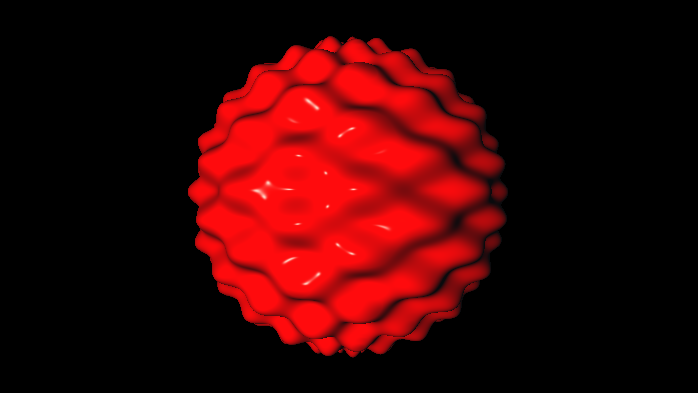
\includegraphics[width=.6\linewidth]{imagens/sdf-distortion/sin-cos-distortion.png}
  \captionof{figure}{Distortion on Sphere from Code 7}
  \label{fig:sin-cos-distortion}
\end{figure}

In Code 7, the Sphere Distance is distorted according to the trigonometric functions applied on its polar and azimutal angle. The result is shown in Figure \ref{fig:sin-cos-distortion}.